\documentclass{article}
% if you need to pass options to natbib, use, e.g.:
%     \PassOptionsToPackage{numbers, compress}{natbib}
% before loading neurips_2026

% The authors should use one of these tracks.
% Before accepting by the NeurIPS conference, select one of the options below.
% 0. "default" for submission
\usepackage{neurips_2026}
% the "default" option is equal to the "main" option, which is used for the Main Track with double-blind reviewing.
% 1. "main" option is used for the Main Track
%  \usepackage[main]{neurips_2026}
% 2. "position" option is used for the Position Paper Track
%  \usepackage[position]{neurips_2026}
% 3. "eandd" option is used for the Evaluations & Datasets Track
 % \usepackage[eandd]{neurips_2026}
 % if you need to opt-in for a single-blind submission in the E&D track:
 %\usepackage[eandd, nonanonymous]{neurips_2026}
% 4. "creativeai" option is used for the Creative AI Track
%  \usepackage[creativeai]{neurips_2026}
% 5. "sglblindworkshop" option is used for the Workshop with single-blind reviewing
 % \usepackage[sglblindworkshop]{neurips_2026}
% 6. "dblblindworkshop" option is used for the Workshop with double-blind reviewing
%  \usepackage[dblblindworkshop]{neurips_2026}

% After being accepted, the authors should add "final" behind the track to compile a camera-ready version.
% 1. Main Track
 % \usepackage[main, final]{neurips_2026}
% 2. Position Paper Track
%  \usepackage[position, final]{neurips_2026}
% 3. Evaluations & Datasets Track
 % \usepackage[eandd, final]{neurips_2026}
% 4. Creative AI Track
%  \usepackage[creativeai, final]{neurips_2026}
% 5. Workshop with single-blind reviewing
%  \usepackage[sglblindworkshop, final]{neurips_2026}
% 6. Workshop with double-blind reviewing
%  \usepackage[dblblindworkshop, final]{neurips_2026}
% Note. For the workshop paper template, both \title{} and \workshoptitle{} are required, with the former indicating the paper title shown in the title and the latter indicating the workshop title displayed in the footnote.
% For workshops (5., 6.), the authors should add the name of the workshop, "\workshoptitle" command is used to set the workshop title.
% \workshoptitle{WORKSHOP TITLE}

% "preprint" option is used for arXiv or other preprint submissions
 % \usepackage[preprint]{neurips_2026}

% to avoid loading the natbib package, add option nonatbib:
%    \usepackage[nonatbib]{neurips_2026}

\usepackage[utf8]{inputenc} % allow utf-8 input
\usepackage[T1]{fontenc}    % use 8-bit T1 fonts
\usepackage{hyperref}       % hyperlinks
\usepackage{url}            % simple URL typesetting
\usepackage{booktabs}       % professional-quality tables
\usepackage{xspace}
\usepackage{amsfonts}       % blackboard math symbols
\usepackage{nicefrac}       % compact symbols for 1/2, etc.
\usepackage{microtype}      % microtypography
\usepackage{xcolor}         % colors
\usepackage{graphicx}
\usepackage{natbib}
\usepackage{multicol}
\usepackage{multirow}
\usepackage{amsmath}
\usepackage[table]{xcolor}
\usepackage{wrapfig}
\usepackage{tikz}
\usepackage[most]{tcolorbox}
\usepackage{alltt}
\usepackage{enumitem}
\usepackage{algorithm}
\usepackage{amssymb}         % For additional math symbols
\usepackage{algpseudocode}   % Provides 'algorithmic' commands like \State, \For, \If
\usepackage{amsmath}         % For math symbols like \mathcal, \text, etc.
\usepackage{cleveref}        % For \cref references to algorithms
\usepackage{pifont}

\newcommand{\cmark}{\ding{51}}
\newcommand{\xmark}{\ding{55}}

\tcbset{
  aibox/.style={
    width=\linewidth,
    top=0pt,
    colback=white,
    colframe=black,
    colbacktitle=black,
    enhanced,
    center,
    attach boxed title to top left={yshift=-0.1in,xshift=0.1in},
    boxed title style={boxrule=0pt,colframe=white,},
  }
}

\usepackage{xspace}
\newcommand{\ours}{CodeClinic\xspace}


\newtcolorbox{AIbox}[2][]{aibox,title=#2,#1}

%% Delete this for anonymity later!!
\newcommand{\draftonly}[1]{#1} 
% Uncomment for submission
% \renewcommand{\draftonly}[1]{}
\newcommand{\draftcomment}[3]{\draftonly{{\textcolor{#3}{[\textbf{#1--\textsc{#2}}]}}}}

\newcommand{\tim}[1]{\draftcomment{#1}{Tim}{teal}}

\newcommand{\junjie}[1]{\draftcomment{#1}{Junjie}{red}}

\title{CodeClinic: Evaluating Compositional Coding Skills for Clinical Reasoning Agents}


% The \author macro works with any number of authors. There are two commands
% used to separate the names and addresses of multiple authors: \And and \AND.
%
% Using \And between authors leaves it to LaTeX to determine where to break the
% lines. Using \AND forces a line break at that point. So, if LaTeX puts 3 of 4
% authors names on the first line, and the last on the second line, try using
% \AND instead of \And before the third author name.


\author{%
  Junjie Hu \\
  University of Wisconsin-Madison \\
  \texttt{\{sluo83, yprabhu2, ossowski, kchen67, junjie.hu\}@wisc.edu} \\
  % examples of more authors
  % \And
  % Coauthor \\
  % Affiliation \\
  % Address \\
  % \texttt{email} \\
  % \AND
  % Coauthor \\
  % Affiliation \\
  % Address \\
  % \texttt{email} \\
  % \And
  % Coauthor \\
  % Affiliation \\
  % Address \\
  % \texttt{email} \\
  % \And
  % Coauthor \\
  % Affiliation \\
  % Address \\
  % \texttt{email} \\
}


\begin{document}


\maketitle


\begin{abstract}
  Recent medical EHR agent systems have equipped LLMs with user-designed tools for retrieving semi-structured clinical data, enabling more accurate and reliable decision-making over complex patient timelines. However, curating these tool libraries requires sustained expert effort, long tool chains incur substantial token overhead, and many clinically meaningful questions remain ill-defined in zero-shot settings due to variability across hospitals and guidelines. We introduce \ours{}, an agentic benchmark built on MIMIC-IV comprising 65k+ instances spanning 260 distinct tasks over 63 clinical concepts. Rather than relying on pre-specified functions, models are encouraged to synthesize modular, reusable tools that capture clinical concepts and compose them to answer complex queries. The benchmark is further stratified by \emph{compositional dependency depth} and includes a \emph{longitudinal} surveillance task that tracks patient state across ICU admissions, making reliable zero-shot resolution incredibly challenging. We show that an offline autoformalization pipeline, which translates clinical guidelines into QA-verified function libraries, substantially outperforms zero-shot code generation, improves generalization across patient populations, and reduces per-query token usage by over 20\%.
\end{abstract}

% \newpage
% \tableofcontents
% \newpage

\section{Introduction}

Large language models (LLMs) have demonstrated remarkable potential for clinical reasoning, achieving expert-level performance on medical licensing examinations~\cite{singhal2023large} and showing strong capabilities across a diverse range of medical tasks~\cite{bedi2025medhelm, wu2025towards, wang2025capabilities}. Recent works have extended these capabilities to agentic settings, where LLMs interact with electronic health record (EHR) databases to answer clinically meaningful questions~\cite{liao2026agentehr, tang2024medagents}. These agents typically generate code or queries to extract structured information from EHR systems and reason over retrieved data to support clinical decisions.

A common approach in these systems is to equip agents with a user-designed toolbox: a curated set of domain-specific functions that the agent can invoke to handle recurring clinical computations. While this strategy improves reliability over purely zero-shot approaches, it does not scale. Designing, validating, and maintaining such toolboxes requires sustained effort from clinical and engineering experts, and the scope of the toolbox is ultimately limited by what its designers anticipated. Moreover, when agents re-execute lengthy tool chains for every complex query, the token cost compounds quickly. This is a practical concern in high-stakes medical deployments where latency and cost matter.

Beyond the toolbox scalability problem, there is a more fundamental issue. Many clinically meaningful questions are simply not well-defined under a zero-shot evaluation regime. Clinical concepts such as sepsis determination, organ failure scoring, and vasopressor thresholds are not universal; their precise operationalizations vary across institutions and evolve with clinical guidelines. An agent answering such questions without access to the relevant institutional definitions faces an underspecified problem, and any benchmark grading its output against a single fixed ground truth will produce misleading accuracy estimates.

These two problems (the fragility of static toolboxes and the ambiguity of zero-shot clinical definitions) point toward a different evaluation paradigm. Rather than asking \emph{how well does an agent answer clinical questions given a fixed toolbox?}, a more scalable and meaningful question is: \emph{given limited verification data, how well can LLMs generate modular, composable libraries for processing EHR data?} If LLMs can reliably synthesize such libraries from clinical guidelines, the bottleneck of expert-curated toolboxes is removed, and the generated code itself encodes the institutional definitions needed to make questions well-posed.

We introduce \textbf{\ours{}}, a benchmark designed to evaluate exactly this capability. \ours{} is grounded in MIMIC-IV~\cite{johnson2020mimic} and spans 63 clinical concepts across nine domains, including severity scores, sepsis criteria, organ failure indices, and ICU treatments. It contains 259 question variants and 63{,}000 QA pairs with difficulty stratified by \emph{compositional dependency depth}, defined as the number of concept-to-concept dependencies an agent must resolve. Crucially, \ours{} also includes a \emph{longitudinal reasoning} component that evaluates agents on questions tracking patient state across the full course of ICU admissions. \junjie{Highlight the key data statistics on the longitudinal agentic task. Should we call it ``longitudinal agentic automation'' instead of ``logitudinal reasoning''?} Both of these properties make the questions genuinely difficult to resolve zero-shot: compositional questions require chaining multi-step computations that naive approaches repeatedly reinvent, while longitudinal questions require consistent state-tracking logic that zero-shot code generation rarely produces reliably. Together, they establish a setting where the quality of an agent's underlying function library, rather than its in-context reasoning alone, is the primary determinant of performance.

To establish a strong baseline, we propose an offline autoformalization pipeline that converts natural-language clinical guidelines into a reusable, QA-verified Python function library via iterative LLM generation. This library is constructed once using limited verification labels, then reused across all queries, eliminating redundant computation and enforcing consistent definitions across runs.

Our contributions are as follows:
\begin{itemize}
\item \textbf{\ours\ (Benchmark)}: 63 clinical concepts, 259 question variants, and 63{,}000 QA pairs derived from MIMIC-IV, with difficulty stratified by compositional dependency depth and a longitudinal reasoning component. The benchmark is designed to surface the failure modes of static toolboxes and zero-shot code generation on questions that are difficult to define without institutional context.
\item \textbf{Benchmark Analysis (Findings)}: A systematic characterization of where and why current LLMs fail on compositional and longitudinal clinical reasoning, including analyses by difficulty level, question type, model scale, and EHR schema familiarity.
\item \textbf{Clinical Autoformalization (Baseline)}: An automated pipeline that transforms natural-language clinical guidelines into a verified Python function library using limited verification data, demonstrating a scalable alternative to user-designed toolboxes and serving as a strong baseline for future work on \ours{}.
\end{itemize}

\section{Related Work}
\begin{table}[t]
\centering
\caption{Comparison of EHR benchmarks relevant to clinical reasoning and agentic evaluation.
\textbf{Code Gen.}: requires generating executable code or SQL.
\textbf{Scale} ($>$10K): $>$10{,}000 QA instances.
\textbf{Agentic}: supports iterative agent loop with execution feedback.
\textbf{Compositional}: explicitly tests multi-hop reasoning over dependent clinical concepts.
\textbf{Longitudinal}: evaluates reasoning over patient state as it evolves over time.}
\label{tab:benchmark_comparison}
\resizebox{\textwidth}{!}{%
\begin{tabular}{lccccc}
\toprule
\textbf{Benchmark} &
\textbf{Code Gen.} &
\textbf{Scale ($>$10K)} &
\textbf{Agentic} &
\textbf{Compositional} &
\textbf{Longitudinal} \\
\midrule
MIMICSQL~\cite{wang2020treqs}          & \cmark & \cmark & \xmark & \xmark & \xmark \\
EHRSQL~\cite{lee2022ehrsql}            & \cmark & \xmark & \xmark & \xmark & \xmark \\
DrugEHRQA~\cite{bardhan-etal-2022-drugehrqa} & \cmark & \cmark & \xmark & \xmark & \xmark \\
EHRXQA~\cite{bae2023ehrxqa}            & \cmark & \xmark & \xmark & \xmark & \xmark \\
EHR-SeqSQL~\cite{bae2024ehrseqsql}    & \cmark & \xmark & \cmark & \xmark & \xmark \\
EHRNoteQA~\cite{kim2024ehrnoteqa}     & \xmark & \xmark & \xmark & \xmark & \xmark \\
EHRAgent~\cite{shi2024ehragent}       & \cmark & \xmark & \cmark & \xmark & \xmark \\
MedAgentGym~\cite{xu2025medagentgym}  & \cmark & \cmark & \cmark & \xmark & \xmark \\
MedAgentBench~\cite{kim2025medagentbench} & \xmark & \xmark & \cmark & \xmark & \xmark \\
AgentClinic~\cite{schmidgall2024agentclinic} & \xmark & \xmark & \cmark & \xmark & \xmark \\
EHRStruct~\cite{zhang2025ehrstruct}   & \cmark & \xmark & \xmark & \xmark & \xmark \\
AgentEHR~\cite{liao2026agentehr}      & \xmark & \cmark & \cmark & \xmark & \xmark \\
EHRSHOT~\cite{wornow2023ehrshot}      & \xmark & \cmark & \xmark & \xmark & \xmark \\
\midrule
\textbf{\ours{} (ours)} & \cmark & \cmark & \cmark & \cmark & \cmark \\
\bottomrule
\end{tabular}%
}
\end{table}
\paragraph{EHR Databases and Benchmarks}
The MIMIC database family is the standard resource for EHR research~\cite{johnson2020mimic, johnson2018mimic}. Early text-to-SQL benchmarks over MIMIC-III such as MIMICSQL~\cite{wang2020treqs} and EHRSQL~\cite{lee2022ehrsql} rely on templated or clinician-collected SQL and cover a constrained query space. EHR-SeqSQL~\cite{bae2024ehrseqsql} extends this to multi-turn SQL interactions. Beyond SQL, DrugEHRQA~\cite{bardhan-etal-2022-drugehrqa} provides 70K medication-focused QA pairs over MIMIC-III spanning both structured tables and free-text notes, while EHRXQA~\cite{bae2023ehrxqa} introduces multimodal QA over MIMIC-IV by coupling structured records with chest X-ray images. EHRNoteQA~\cite{kim2024ehrnoteqa} targets free-text discharge summaries, requiring synthesis across multiple clinical notes. EHRSHOT~\cite{wornow2023ehrshot} provides 15 few-shot clinical prediction tasks over longitudinal Stanford EHR data, evaluating foundation models on structured time-series inputs, though tasks are point-in-time predictions rather than agent reasoning. On the code-generation side, EHRAgent~\cite{shi2024ehragent} frames complex tabular EHR reasoning as iterative code generation with execution feedback, and EHRStruct~\cite{zhang2025ehrstruct} benchmarks 11 structured-data tasks spanning retrieval, aggregation, and temporal reasoning over Synthea and eICU. Across these works, evaluation is conducted over static, individually posed queries; none provides mechanisms to assess multi-hop concept dependencies or time-evolving clinical state. Furthermore, all prior benchmarks that involve tool use rely on toolboxes pre-designed by domain experts, leaving open the question of whether LLMs can autonomously generate the libraries needed to answer such questions. Table~\ref{tab:benchmark_comparison} summarizes how these benchmarks compare. \ours{} is the only benchmark to jointly support compositional difficulty stratification (via explicit dependency-chain depth across 63 clinical concepts) and longitudinal reasoning over patient trajectories.

\paragraph{LLM-Based Medical Agents}
Several agent systems interact with EHR data to support clinical decisions~\cite{liao2026agentehr, tang2024medagents, hager2024evaluation, bani2025language}. MedAgentGym~\cite{xu2025medagentgym} provides a code-based gym for training medical agents but requires a separately curated environment per task. Biomni~\cite{huang2025biomni} discovers biomedical tools from literature but relies on large proprietary LLMs with no training. MedAgentBench~\cite{kim2025medagentbench} evaluates agents against a realistic FHIR-based virtual EHR environment with 300 tasks spanning ten clinical categories, while AgentClinic~\cite{schmidgall2024agentclinic} tests multi-turn diagnostic reasoning through simulated patient interaction. A key limitation shared across these systems is the reliance on user-designed tool environments: the clinical functions agents invoke are hand-crafted by researchers, making evaluation contingent on the completeness and correctness of those tools. This design also incurs significant token overhead when agents must re-execute full tool chains for each new query. Broad evaluations such as MedHELM~\cite{bedi2025medhelm, bedi2026holistic} assess static task performance without agentic EHR interaction. Our work is orthogonal. Rather than evaluating an agent's behavior within a fixed tool environment, we ask how well LLMs can generate the tool environment itself.

\paragraph{Autoformalization and Code-Augmented Reasoning}
Autoformalization, the translation of informal statements into formal, executable representations, was demonstrated for mathematics by Wu et al.~\cite{wu2022autoformalization} using LLMs to translate theorems into Lean and Isabelle. We adapt this concept to clinical guidelines, replacing proof checkers with QA-based verification and targeting a Python function library rather than formal proofs. This reframing is key: unlike mathematical theorems, clinical guidelines encode institutional norms that vary across hospitals, so the formalization process itself resolves the definitional ambiguity that makes zero-shot evaluation unreliable. On the reasoning side, ReACT~\cite{yao2023react} showed that interleaving reasoning with tool calls improves agent performance, and program-aided approaches such as PAL~\cite{gao2023pal} and Codex~\cite{chen2021codex} demonstrate the value of code as a reasoning medium. Our approach uses a ReACT-style loop \emph{offline} to generate a stable, reusable function library, separating the costly library-construction phase from inference and avoiding the repeated token expenditure of agents that re-derive the same computations at query time.

\section{Benchmark}

\subsection{MIMIC Compositional QA}
\begin{figure}[t]
    \centering
    \begin{minipage}{0.48\linewidth}
    \centering
    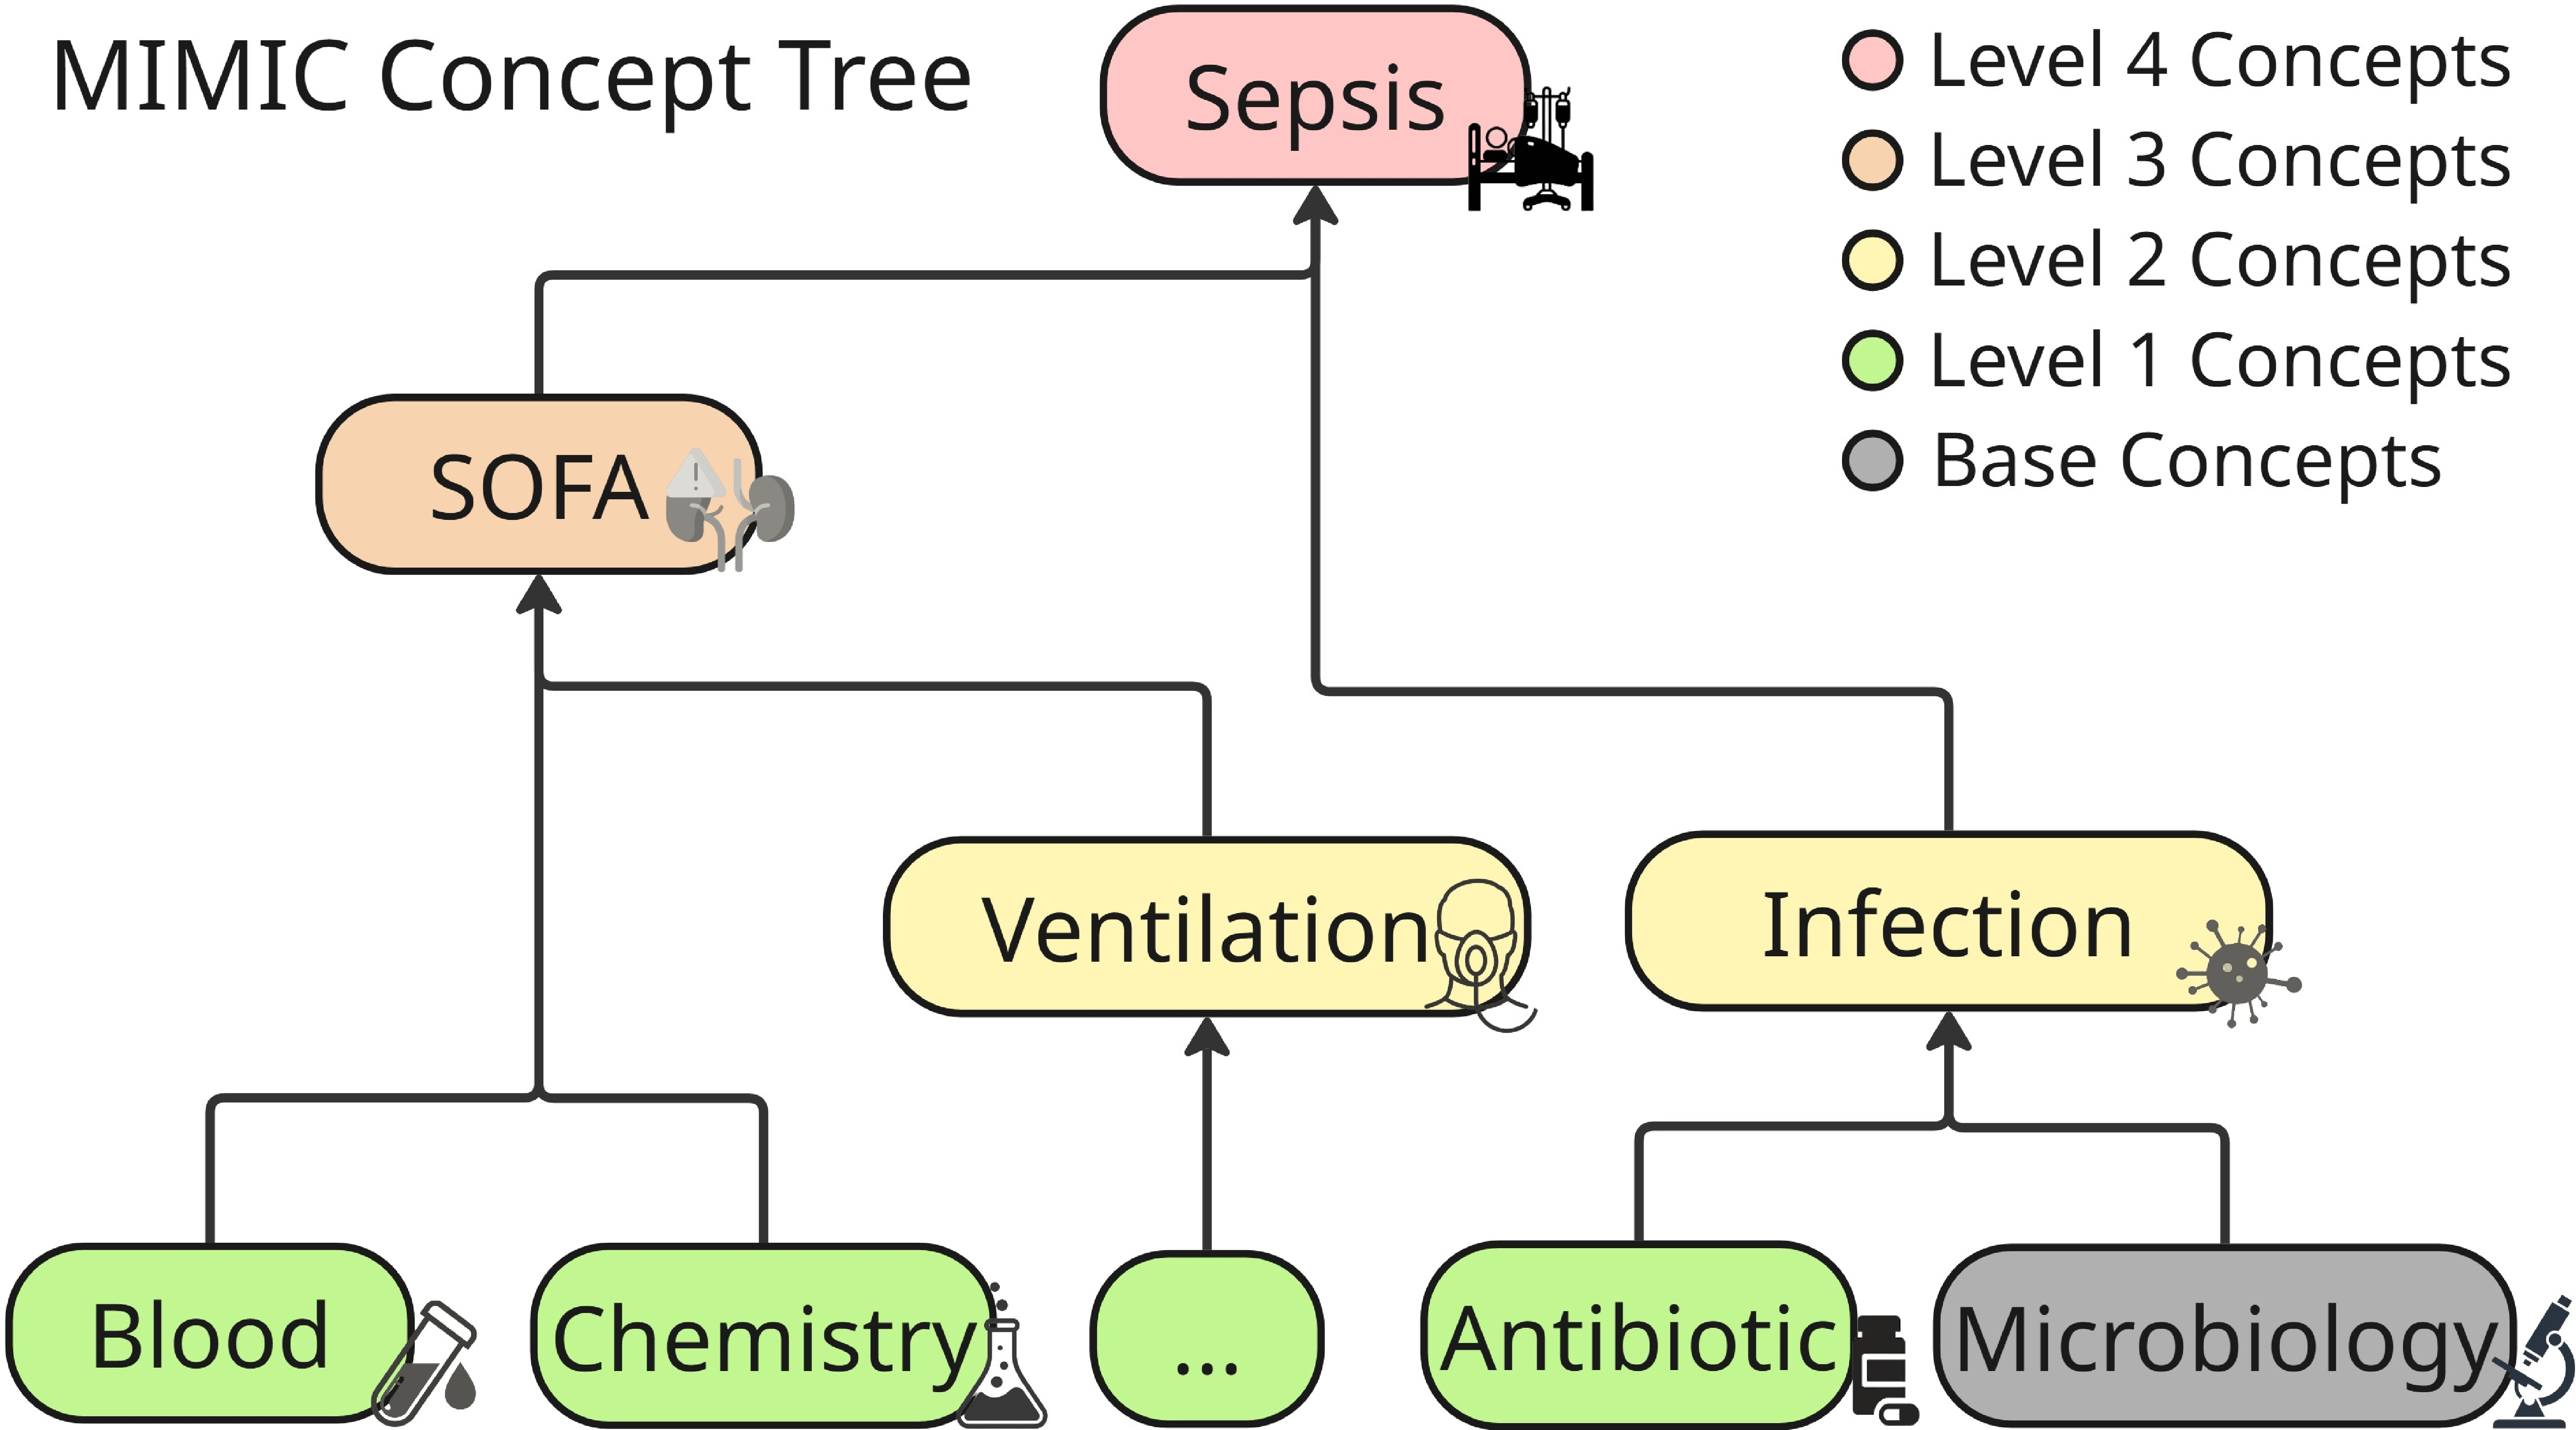
\includegraphics[width=\linewidth]{figures/dependency_example.pdf}
    \end{minipage}
    \begin{minipage}{0.48\linewidth}
        \centering
        \raisebox{13mm}{
            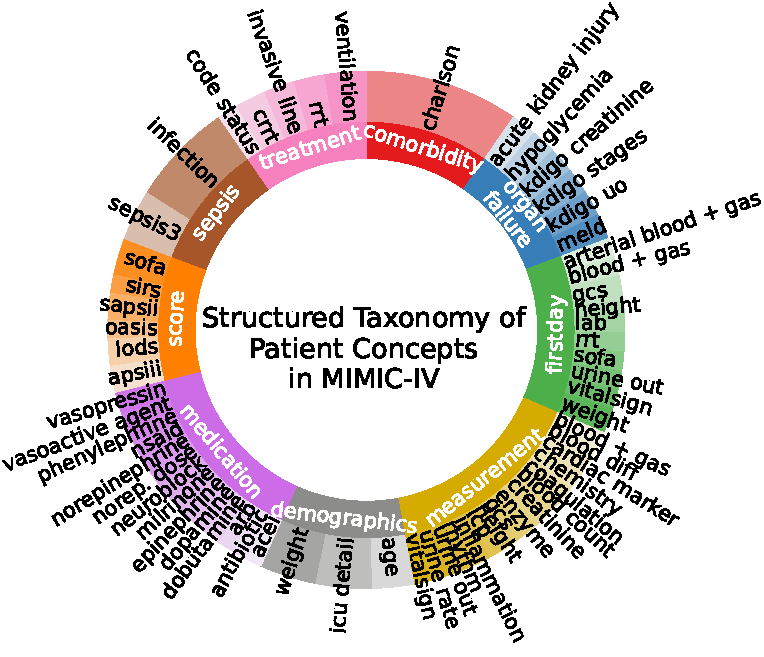
\includegraphics[width=\linewidth]{figures/concept_distribution.pdf}
        }
    \end{minipage}
    \vspace{-15mm}
    \caption{
    \textbf{Left:} Example dependency tree between clinical concepts in the MIMIC database for Sepsis. 
    Efficient sepsis monitoring involves recalculation of lower level concepts such as SOFA, Infection, etc. 
    \textbf{Right:} Structured taxonomy of all MIMIC concepts supercategories and corresponding concepts.
    }
    \label{fig:dependency_with_table}
\end{figure}
We constructed a clinical question answering benchmark grounded in the Medical Information Mart for Intensive Care IV (MIMIC-IV) database~\cite{johnson2023mimic}. All questions are derived from structured data in the MIMIC-IV \texttt{derived} schema, a curated collection of tables produced by community-validated SQL transformations applied to the raw MIMIC-IV data~\cite{johnson2021mimic}. The benchmark spans 63 clinical concepts covering nine physiological and pharmacological domains: comorbidity scoring, patient demographics, first-day assessments, laboratory measurements, medication administration, organ failure indices, severity scores, sepsis-related variables, and ICU treatments.

\paragraph{Concept Definition} Each concept corresponds to one derived table (e.g., \texttt{sofa}, \texttt{ventilation}, \texttt{kdigo\_stages}) and is defined programmatically as a set of question variants paired with ground-truth extraction functions. Each concept specifies (i) a base SQL query that joins the derived table with \texttt{mimiciv\_icu.icustays} and \texttt{mimiciv\_hosp.admissions} to produce a per-stay feature matrix, and (ii) a set of question variants, each targeting a distinct clinical attribute and question type. For each concept we also generate a structured natural-language guideline specification (defining clinical criteria, required measurements, and temporal windows) by synthesizing PubMed literature with an LLM (details in Appendix~\ref{app:guideline_gen}).

\paragraph{Clinical Knowledge Graph.}
Concepts are organized into a directed acyclic dependency graph $\mathcal{G} = (V, E)$, where an edge $(v_i, v_j)$ indicates that $v_j$ requires output from $v_i$. The graph is constructed by parsing SQL definitions in the MIMIC-Code repository and expanding with clinical conditions derived from ICD-10 diagnoses and UMLS Metathesaurus relations (see Appendix~\ref{app:knowledge_graph} for full construction details). This structure drives both difficulty stratification and compositional function reuse in our baseline pipeline.
\paragraph{Dependency-Based Difficulty} A key property of MIMIC-IV derived tables is that many are computed from other derived tables, inducing a directed acyclic dependency graph. We assign each concept a difficulty level equal to its longest dependency-chain depth in this graph. Concepts with no upstream dependencies (e.g., \texttt{vitalsign}, \texttt{gcs}, \texttt{norepinephrine}) are assigned \textit{Level 1}; these represent raw chart-level or medication-level extractions that require no multi-table reasoning. Concepts at depth 2 (e.g., \texttt{ventilation}, \texttt{creatinine\_baseline}, \texttt{first\_day\_lab}) are assigned \textit{Level 2}; they aggregate one layer of derived tables and correspond to clinically interpreted quantities. Concepts at depth 3 or greater (e.g., \texttt{sofa} at depth 3, \texttt{sepsis3} at depth 4) are grouped as \textit{Level 3+}; these composite scores integrate information across many physiological sub-systems and require reasoning over the most derived clinical constructs. This stratification provides a natural proxy for reasoning difficulty: correctly answering questions about a sepsis determination requires implicitly reasoning about organ dysfunction scores, infection likelihood, antibiotic timing, and microbiological culture data, a fundamentally more complex inference chain than answering questions about raw vital signs. We provide a visual representation of these dependencies in Figure \ref{fig:dependency_with_table}

% \paragraph{Question Types} We define question variants spanning four types for each concept. \textit{Binary} (yes/no) questions ask whether a clinical threshold is met or an event occurred (e.g., Does this patient have a SOFA score of 2 or more during their first 24 hours in the ICU?''). \textit{Numerical} questions require retrieving or computing a precise scalar value (e.g., What is this patient's minimum GCS score on their first ICU day?''). \textit{Temporal} questions test time-bounded reasoning by asking about measurements or events within a specific window relative to ICU admission (e.g., Was this patient's urine output rate below 0.5~mL/kg/hr within the first 6 hours of ICU admission?''); these are implemented via inline SQL \texttt{INTERVAL} expressions (6, 12, or 24 hours). \textit{Categorical} questions require predicting a discrete label from a multi-valued output space (e.g., Which ICU unit was this patient first admitted to?''). Across all 63 concepts, the benchmark contains 259 unique question phrasings (143 binary, 51 numerical, 58 temporal, 7 categorical).

\textbf{Sampling and Splits.} For each concept, up to 200 ICU stays are sampled per variant with class balance (100 positive / 100 negative for binary questions); no subject appears in more than one variant within a concept. A 10\% subset (20 rows per variant) forms the training split used during autoformalization; the remaining 90\% is the held-out test set. The full benchmark comprises \textbf{63,000 QA pairs} across 42,311 unique ICU stays (6,300 train / 56,700 test). Ground-truth labels are extracted deterministically from derived tables; missing values (e.g., no ICP measurements) are labeled \texttt{NaN} and a model correctly reporting data absence is scored correct.

\subsection{Longitudinal Reasoning}
{\color{blue}
We complement the static compositional QA benchmark with a longitudinal ICU surveillance task that evaluates whether an agent can maintain clinically consistent state over time rather than answer a single isolated question. The source cohort contains all MIMIC-IV ICU stays with length of stay at least 48 hours, yielding 46{,}337 stays and 602{,}381 checkpoint rows. We sample checkpoints every 4 hours from ICU admission through hour 48, so each trajectory contains 13 decision points. The public benchmark package is a held-out 2{,}000-stay subset (400 dev, 1{,}600 test; 26{,}000 checkpoints) selected from the cohort using a soft-balancing policy that preserves ICU heterogeneity while enriching rare high-acuity states.

\begin{figure}[t]
    \centering
    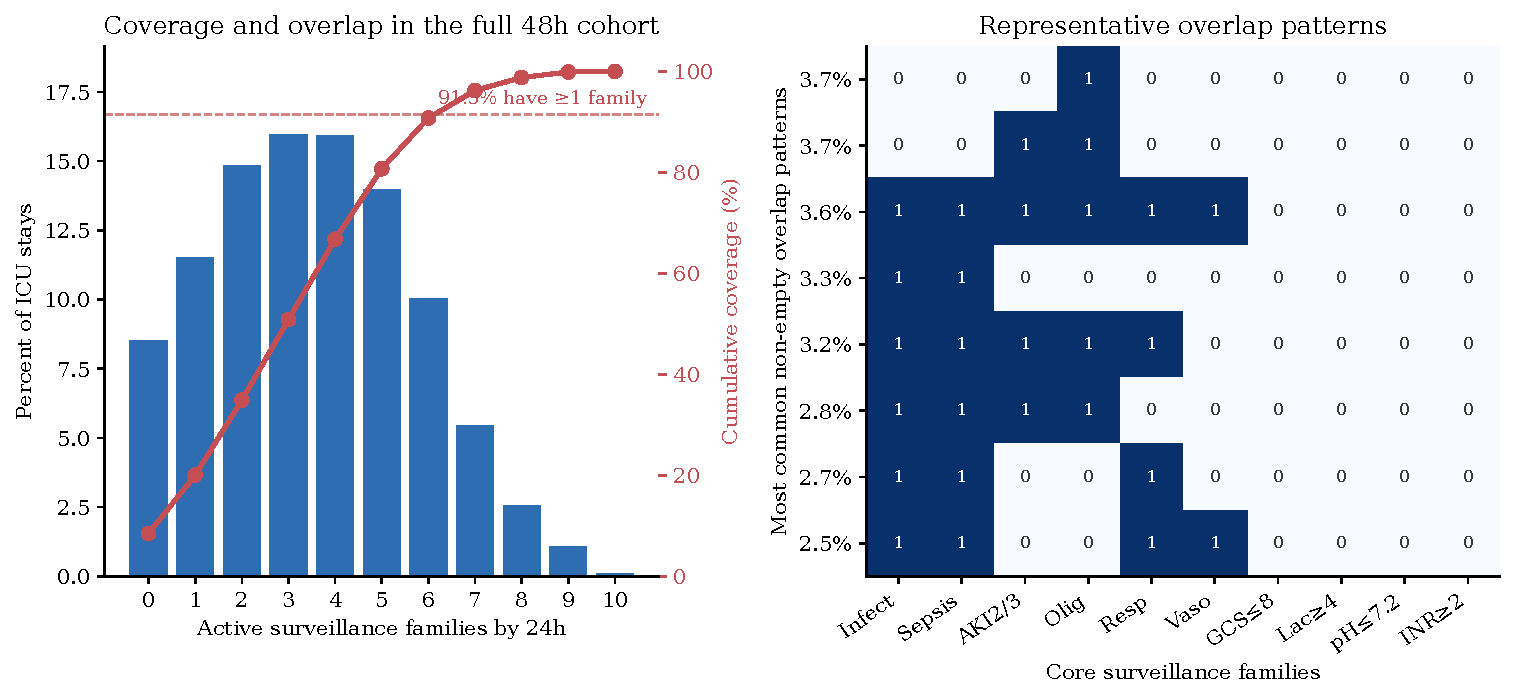
\includegraphics[width=\linewidth]{figures/surveillance_overlap_coverage.pdf}
    \caption{\textcolor{blue}{Coverage and overlap statistics for the longitudinal surveillance cohort. Left: distribution of the number of active core surveillance families by 24 hours among ICU stays with length of stay $\geq 48$ hours. Right: the most common non-empty overlap patterns across the ten core families, showing that many trajectories contain multiple concurrent monitoring problems rather than a single isolated disease.}}
    \label{fig:surveillance_coverage}
\end{figure}

Each checkpoint is labeled in two layers. Internally, we maintain a latent registry of 25 canonical ICU surveillance decisions spanning eight families: infection, sepsis, renal, respiratory, hemodynamic, neurologic, metabolic, and coagulation. Externally, these decisions are compressed into a simple agent output interface consisting of \texttt{suspected\_conditions}, \texttt{alerts}, \texttt{global\_action}, and \texttt{priority}. Importantly, these labels are not governed by a single one-time-trigger rule. Instead, the ground truth follows disease-appropriate checkpoint semantics derived from MIMIC-IV clinical principles: infection and sepsis are persistent episode states once they begin, AKI uses cumulative maximum-stage semantics, ventilation and vasoactive support are active-interval states, recent physiologic abnormalities such as lactate, pH, GCS, PF ratio, INR, and oliguria use recency-based TTL windows, and composite states such as septic shock are recomputed at every checkpoint from their component evidence.

\begin{figure}[t]
    \centering
    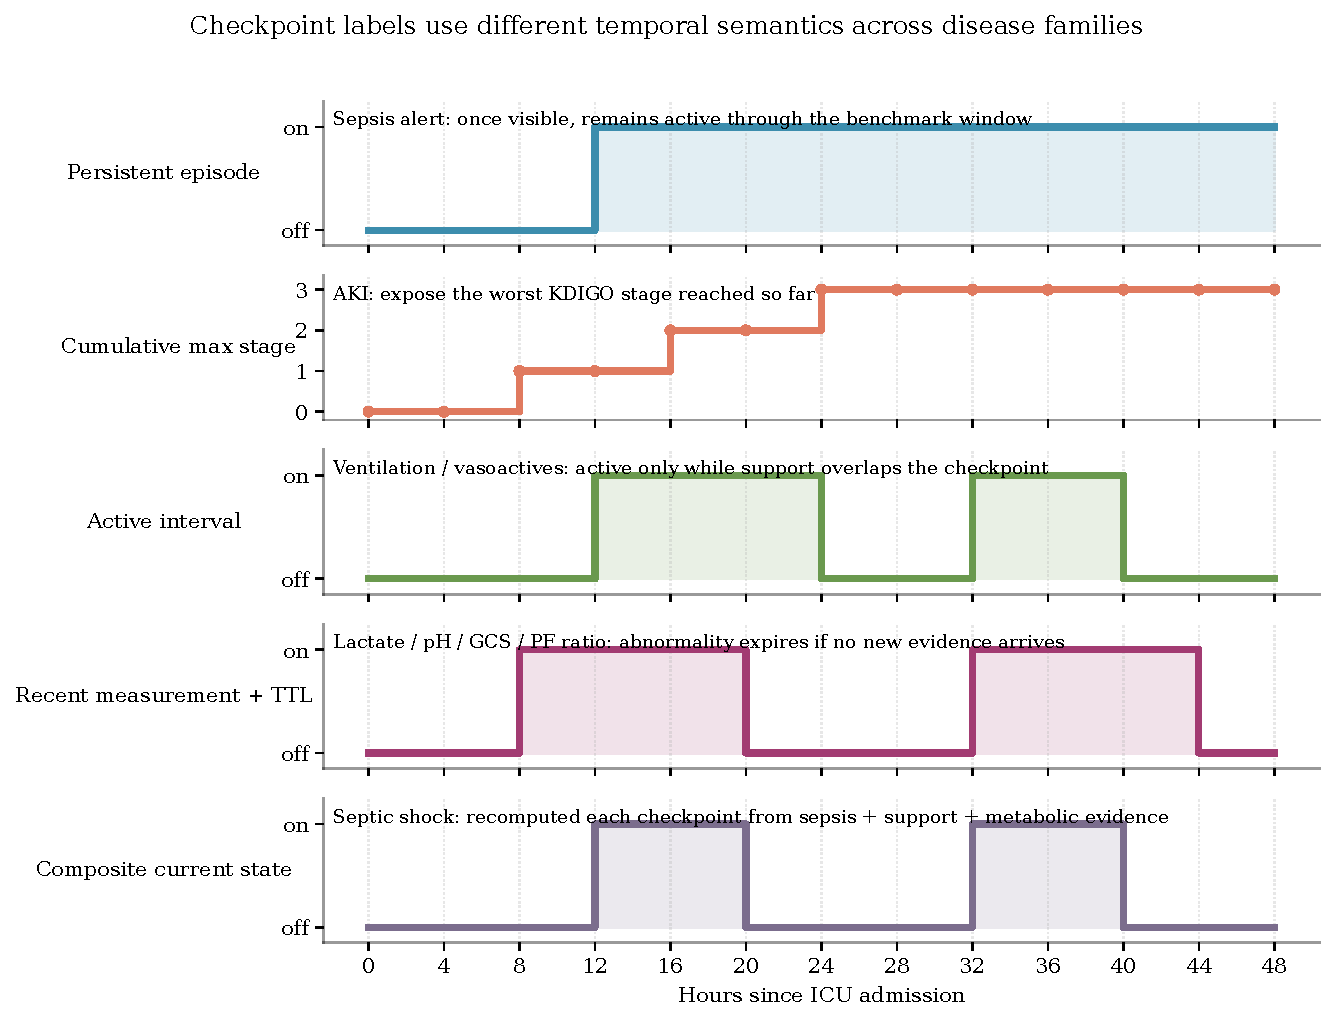
\includegraphics[width=\linewidth]{figures/surveillance_state_semantics.pdf}
    \caption{\textcolor{blue}{The longitudinal benchmark uses disease-dependent checkpoint semantics rather than a uniform once-positive-forever rule. Persistent syndromes such as sepsis remain active after onset; AKI tracks the worst KDIGO stage reached so far; support therapies such as ventilation and vasoactives are active only while the intervention overlaps the checkpoint; recent physiologic abnormalities such as lactate, pH, GCS, PF ratio, and oliguria expire after task-specific TTL windows; and composite states such as septic shock are recomputed from their component evidence at every checkpoint.}}
    \label{fig:surveillance_semantics}
\end{figure}

This temporal heterogeneity is a core source of difficulty. A model cannot solve the task by remembering a single binary label per disease. It must instead track which families persist once triggered, which families should decay when evidence becomes stale, and which families must be recomputed from multiple evolving components. For example, infection suspicion and Sepsis-3 onset remain active after they first occur within the 48-hour window; AKI is exposed as the worst KDIGO stage reached so far rather than the latest row value; invasive ventilation and vasoactive support are active only while the intervention overlaps the current checkpoint; oliguria and severe oliguria use rolling 6-hour and 24-hour windows; GCS states expire after 8 hours; blood-gas-derived states such as PF ratio, lactate, and acidemia expire after 12 hours; INR-based coagulation states expire after 24 hours; and septic shock or shock-with-hypoperfusion are recomputed from the conjunction of sepsis, support, and metabolic evidence. Figure~\ref{fig:surveillance_semantics} illustrates these distinct state-transition patterns.

This design makes the surveillance task both broad and genuinely longitudinal. In the full cohort, 91.49\% of stays activate at least one core surveillance family by 24 hours, 79.96\% activate at least two, and 65.10\% activate at least three; only 8.51\% remain negative across all ten core families at 24 hours (Figure~\ref{fig:surveillance_coverage}). The decision space also spans both common and rare ICU states. By 24 hours, for example, 51.23\% of stays meet Sepsis-3 criteria, 46.74\% receive invasive ventilation, 34.06\% receive vasoactive support, 17.33\% have PF ratio $<100$, 10.65\% have severe acidemia, and 1.91\% receive CRRT. To avoid a benchmark dominated by the most common alerts, the released 2{,}000-stay subset mixes 1{,}200 \emph{core-diversity} stays, 600 \emph{alert-enrichment} stays, and 200 \emph{low-signal} stays. This preserves realistic co-occurrence structure while ensuring enough support for thinner but clinically important heads such as AKI stage 3 (325 stays), septic shock (350), shock with hypoperfusion (280), severe acidemia (212), and severe coagulopathy (240).

At inference time, an agent is prompted at each checkpoint with the current hour, compact summary memory from prior steps, and access to one of two benchmark interfaces over the same time-bounded DuckDB session: a Python-session mode or a tool-first retrieval mode. In both cases the agent must retrieve any needed guideline or function evidence, infer the patient's current ICU state, emit a structured surveillance decision, and then summarize the step for future checkpoints. This setup turns longitudinal reasoning into an agentic state-tracking problem: the model must decide what clinical evidence to gather, how to interpret evolving partial observations, and when to escalate from monitoring to alerting without access to the full future trajectory.
}


\begin{figure}[!t]
    \centering
    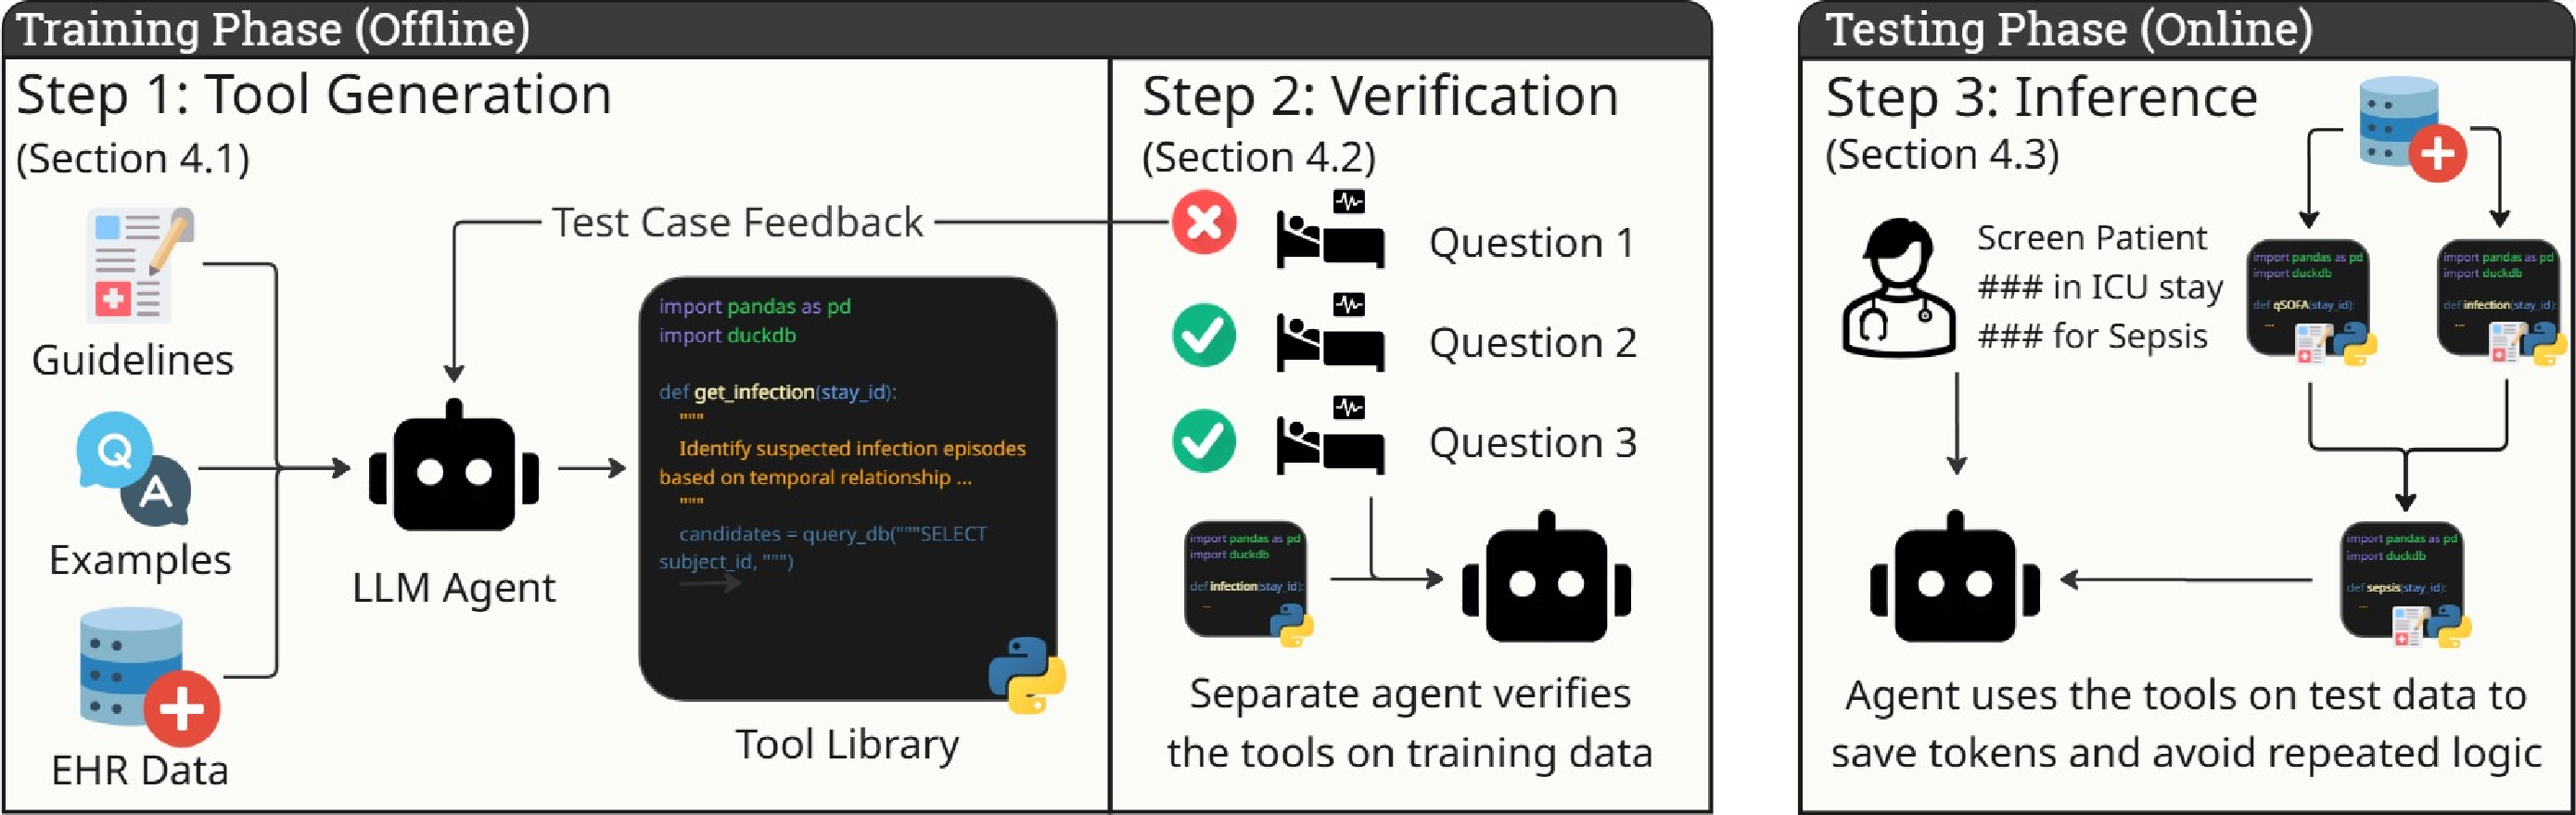
\includegraphics[width=\linewidth]{figures/pipeline.pdf}
    \caption{Overview of the clinical autoformalization pipeline. An LLM agent iteratively explores the EHR schema, consults clinical guidelines, and refines a Python function until it passes QA-based verification. Verified functions are stored in a shared library and reused compositionally for higher-level and new tasks.}
    \label{fig:pipeline}
\end{figure}

\begin{figure}[!h]
    \centering
    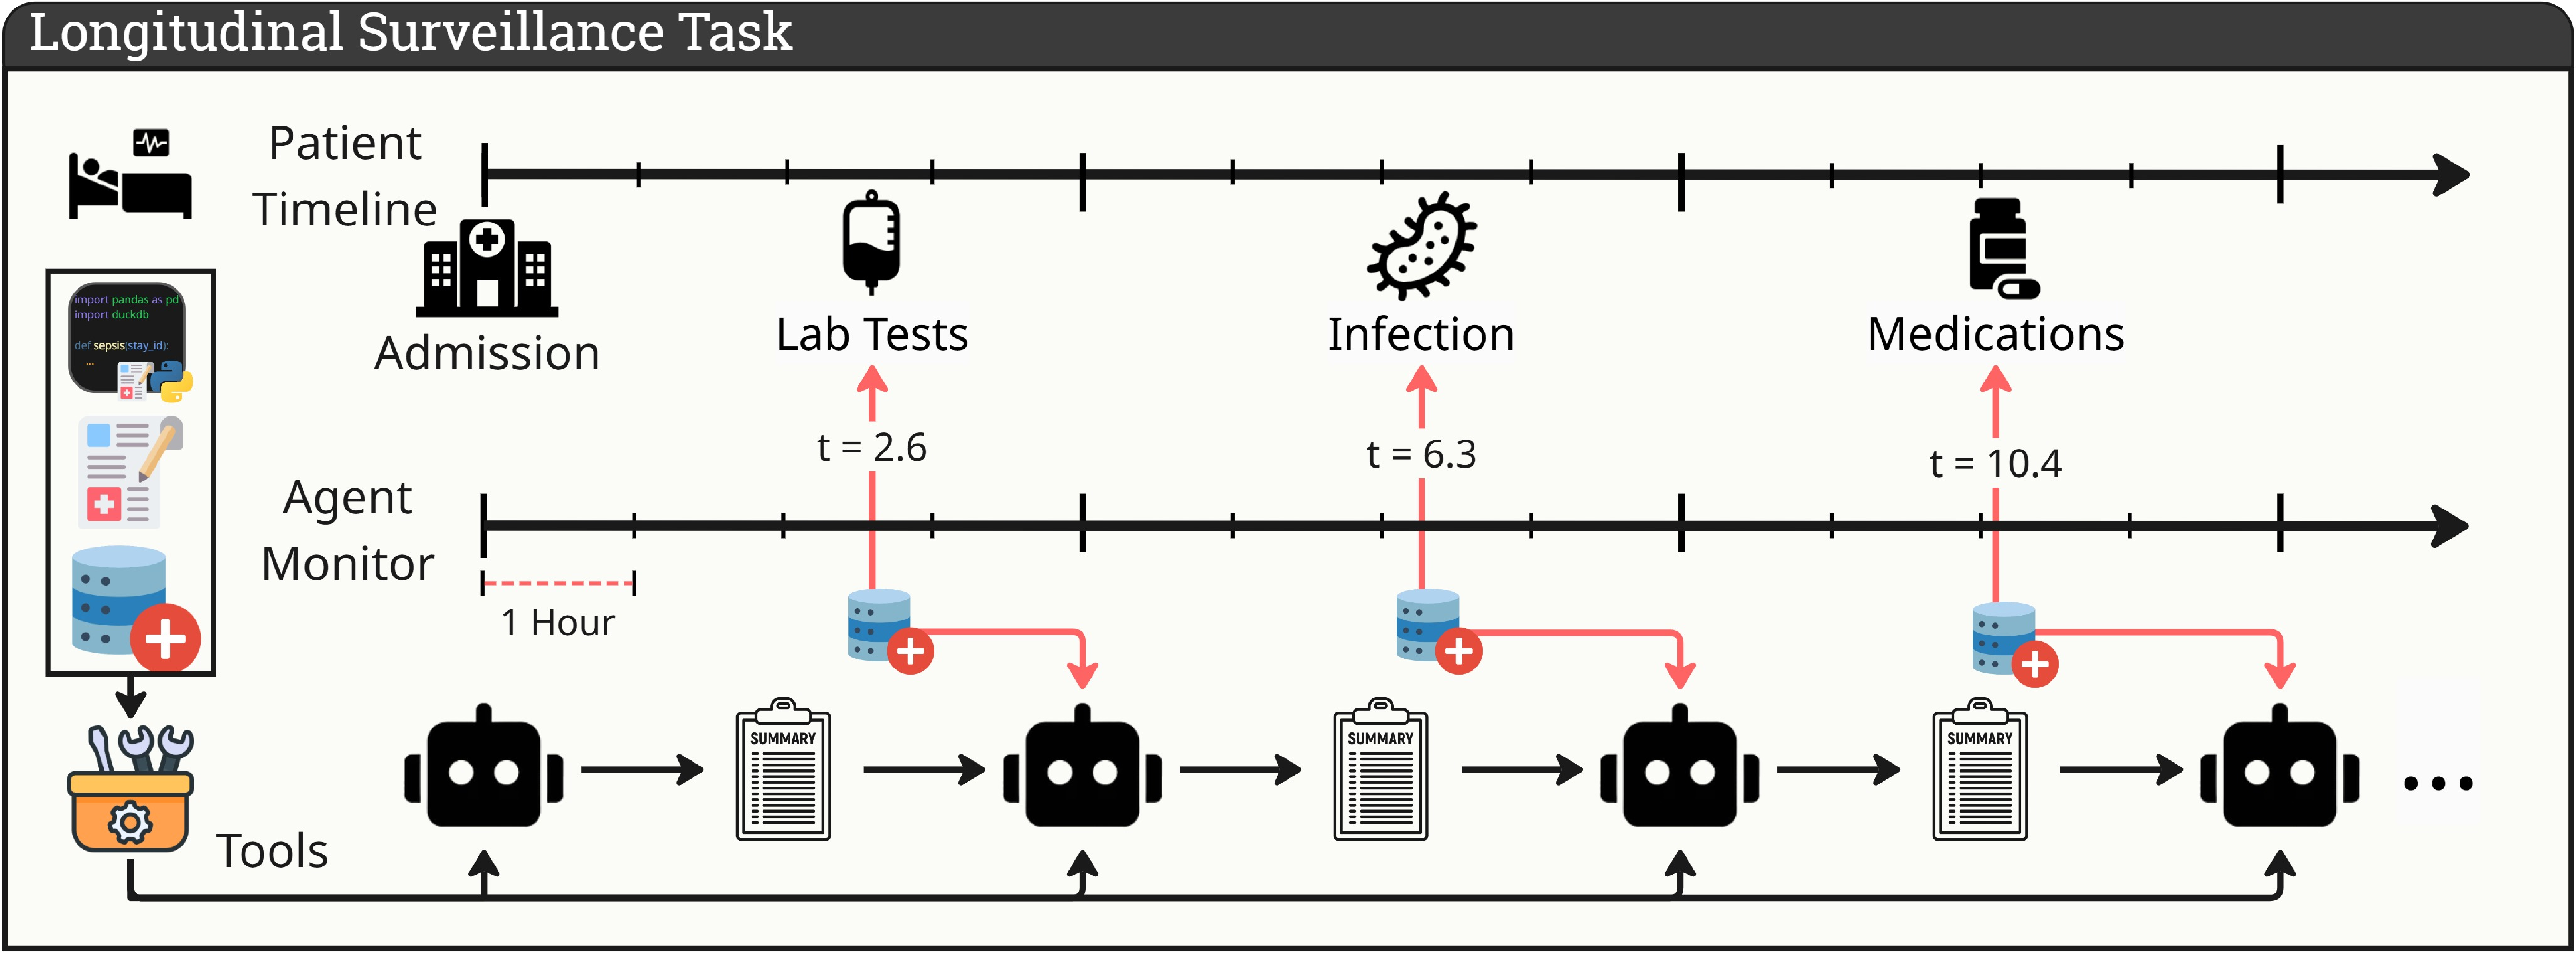
\includegraphics[width=\linewidth]{figures/longitudinal_pipeline.pdf}
    \caption{Overview of the longitudinal patient surveillance task in our benchmark. The LLM agent is prompted every 4 hours to predict patient condition and summarize.}
    \label{fig:longitudinal}
\end{figure}


\section{Baseline: Clinical Autoformalization}


We propose a clinical autoformalization pipeline that converts natural-language clinical guidelines into a verified, reusable Python function library using only a small train split as supervision. The pipeline takes as input a QA dataset $\mathcal{Q} = \{(q_k, y_k)\}_{k=1}^{K}$, an EHR database $\mathcal{C}$, and clinical guidelines $\mathcal{G}$, and produces a verified Python function $f$ that deterministically extracts a clinical concept for any patient. The full algorithm is given in Appendix~\ref{app:algorithm}.

\subsection{Tool Generation}

The core of the pipeline is an iterative ReACT loop~\cite{yao2023react} in which an LLM agent explores the EHR database schema, consults clinical guidelines, and writes a Python function for a target concept. The agent operates within a stateful code interpreter exposing three tools: \texttt{query\_db(sql)} for database access, \texttt{search\_guidelines}/\texttt{get\_guideline} for retrieving clinical specifications from $\mathcal{G}$, and \texttt{search\_functions}/\texttt{load\_function} for discovering and importing previously verified functions. Guidelines are exposed as a searchable library rather than injected into the prompt, forcing the agent to bridge clinical knowledge and database schema through autonomous exploration.

Concepts are processed in topological order over the dependency graph $G = (V, E)$, where $(v_i, v_j) \in E$ means $v_j$ depends on $v_i$. Leaf concepts are autoformalized first; higher-level concepts can then call previously verified functions as building blocks rather than reimplementing their logic. For example, when generating a function for \texttt{sepsis3}, the agent can load verified functions for \texttt{sofa} and \texttt{suspicion\_of\_infection} directly.

\subsection{Verification}

Once the agent produces a candidate function $f_t$, it is evaluated against the 10\% train split of $\mathcal{Q}$. A separate QA agent calls $f_t$ in its own code interpreter and parses a verdict for each question to compare against ground truth. If accuracy exceeds $\theta = 0.90$, the function is accepted and saved to the shared library. Otherwise, per-question error traces are fed back to the autoformalization agent as structured feedback for the next iteration. The best-performing candidate across all iterations is retained, so the pipeline is robust to minor regressions between steps.

\subsection{Inference}

Once the library $\mathcal{L} = \{f_1, \dots, f_M\}$ is complete, it is deployed as a static resource over the held-out 90\% test split. An LLM inference agent receives a clinical question $q$ along with access to $\mathcal{L}$ and the database, calls the relevant pre-verified functions according to its judgment, and reasons over their outputs to produce an answer:
\begin{equation}
    \hat{y} = \text{LLM}\bigl(q,\; \{f_j(p) : f_j \in \mathcal{L}\},\; \mathcal{C}\bigr)
\end{equation}
Because the functions in $\mathcal{L}$ have been verified on labeled cases, the inference agent's context is occupied by compact function signatures rather than raw schema exploration, substantially reducing token usage. The same function produces identical output for the same patient across runs, which is critical for reproducibility in clinical settings.

\section{Results}

\begin{figure}
    \centering
    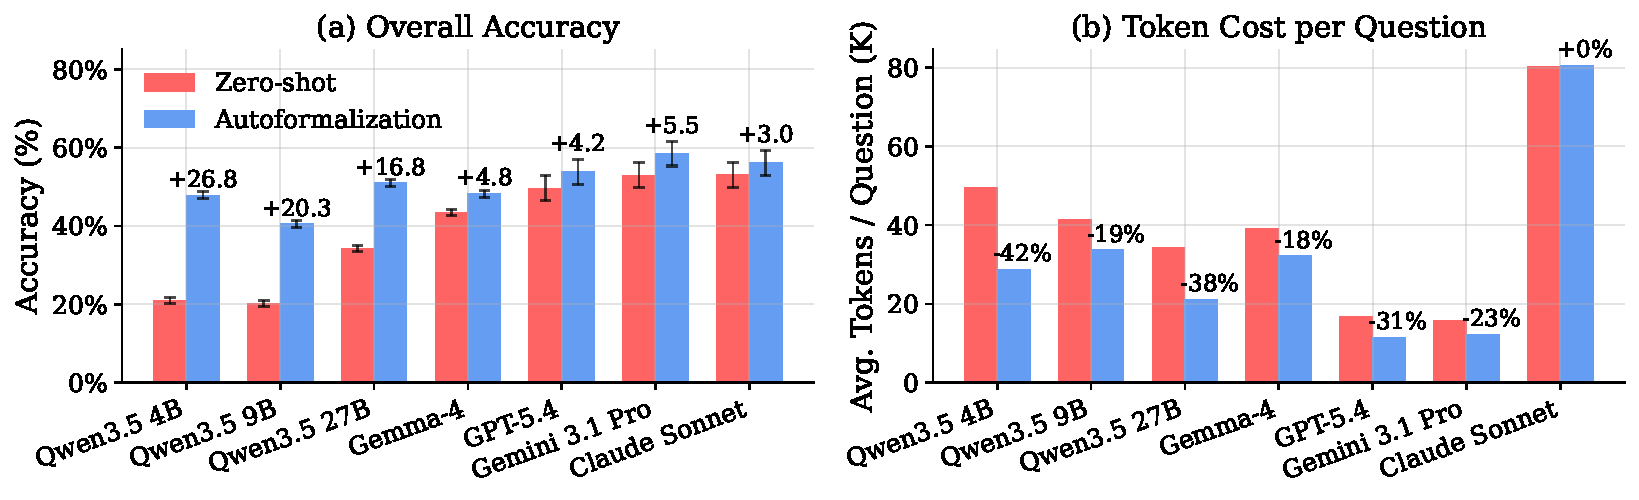
\includegraphics[width=1\linewidth]{figures/comparison_overall.pdf}
    \caption{Caption}
    \label{fig:placeholder}
\end{figure}

We organize our experimental evaluation around three questions:
(1) How difficult is clinical QA over real EHR databases for current LLMs?
(2) How does clinical autoformalization compare to alternative approaches?
(3) How well do autoformalized libraries generalize across guidelines, databases, and patient populations?
All autoformalization and inference experiments use \texttt{vllm}~\cite{kwon2023efficient} as the inference engine.
The autoformalization loop allows up to 100 exploration turns per concept with a context compression threshold of 25{,}000 tokens; the QA verification and inference agents are limited to 10 turns each.
A stratified subset of 100 patients per concept is used for verification during autoformalization, and evaluation is performed on the held-out 90\% test split (56{,}700 QA pairs).

%% ============================================================
%% 5.1 TASK DIFFICULTY: LLM PERFORMANCE BY DIFFICULTY LEVEL
%% ============================================================
\subsection{Task Difficulty}
\label{sec:task_difficulty}

To characterize the difficulty of \ours{} and establish the landscape for current LLMs, we evaluate a diverse set of models in a zero-shot code-generation setting. Each model is given the raw MIMIC-IV schema, a \texttt{query\_db} function, and a clinical question, and must iteratively generate executable code to retrieve and analyze information from the database. The model can then reason over execution outputs to produce an answer or continue refining its code, for up to 10 iterations. We select models spanning multiple families and scales to ensure broad coverage and to control for potential schema memorization from pretraining data, since MIMIC-IV is a widely studied dataset.

% ---- TABLE 1: LLM performance by difficulty level ----
\begin{table}[t]
\centering

\label{tab:llm_difficulty}
\resizebox{\linewidth}{!}{
\begin{tabular}{lcccccc}
\toprule
\multirow{2}{*}{Model} & \multicolumn{4}{c}{Accuracy by Difficulty Level} & \multirow{2}{*}{Overall} & \multirow{2}{*}{Tokens/Q} \\
\cmidrule(lr){2-5}
& Level 1 & Level 2 & Level 3+ & $\Delta$ (L1$\to$L3+) & & \\

\midrule
\multicolumn{7}{c}{\textbf{Frontier Models}} \\
\midrule

Claude-Sonnet-4.6  & 58.4 & 51.0 & 41.1 & -17.3 & 53.1 & 80308 \\
Gemini-Pro-3.1  & 58.0 & 54.1 & 37.2 & -20.8 & 53.0 & 15897* \\
GPT-5.4  & 55.1 & 47.8 & 36.7 & -18.4 & 49.6 & 16778 \\

\midrule
\multicolumn{7}{c}{\textbf{Open-Source Models}} \\
\midrule

Gemma4-31B        & 46.9 & 44.2 & 32.2 & -14.7 & 43.4 & 39243 \\
gpt-oss-120B      & 39.4 & 38.6 & 23.2 & -16.2 & 36.1 & \textbf{19576} \\
Kimi-K2.6         & 37.1 & 41.6 & 19.7 & -17.4 & 35.0 & 33017 \\
Qwen3.5-27B       & 36.5 & 38.6 & 21.6 & -14.9 & 34.2 & 34414 \\
Qwen3.5-9B        & 22.8 & 22.9 & 8.7 & -14.2 & 20.2 & 41378 \\
Qwen3.5-4B        & 25.4 & 20.9 & 8.6 & -16.8 & 21.0 & 49445 \\

\bottomrule
\end{tabular}
}
\caption{Zero-shot QA accuracy (\%) of LLMs on \ours{} by difficulty level. All models are given only the raw MIMIC-IV schema and a \texttt{query\_db} tool. Difficulty levels correspond to dependency-chain depth in the clinical concept graph (Section~3). Results are averaged across question types within each level.}
\end{table}

Table~\ref{tab:llm_difficulty} reports accuracy across all 63 concepts, grouped by difficulty level.
Several trends emerge.
First, even the strongest frontier models achieve only moderate accuracy overall, confirming that clinical QA over real EHR databases remains a challenging task that is far from saturated.
Second, performance degrades consistently from Level~1 to Level~3+ across all model families, with the drop (column $\Delta$) reflecting the compounding effect of multi-hop dependencies: answering a Sepsis-3 question requires correctly computing SOFA sub-scores, infection criteria, and antibiotic timing, each of which can independently fail.


%% ============================================================
%% 5.2 BASELINE COMPARISONS
%% ============================================================
\subsection{Comparison of Approaches}
\label{sec:baselines}

We compare several agentic setups to isolate the contribution of autoformalized code libraries.
All approaches use the same backbone LLM (\texttt{Qwen-3-4B}) at inference time.

\begin{enumerate}[label=\textbf{(\arabic*)},nosep,leftmargin=*]
    \item \textbf{Raw Schema + \texttt{query\_db}}: The LLM receives only the raw MIMIC-IV schema and a \texttt{query\_db} function. This is the zero-shot baseline from Section~\ref{sec:task_difficulty}.
    \item \textbf{RL Finetuning}: We finetune 3 different Qwen3 models of increasing scale (\texttt{Qwen3-4B}, \texttt{Qwen3-14B}, and \texttt{Qwen3-32B}) \cite{yang2025qwen3} using standard GRPO \cite{shao2024deepseekmath}. During training, the models receive only the MIMIC-IV schema and a \texttt{query\_db function}. We sample 5 training examples per concept for each model's training. Full training parameters are listed in the appendix section \ref{app:train_details}.
    \item \textbf{Clinical Autoformalization (Ours)}: The LLM is given the raw MIMIC-IV schema, a \texttt{query\_db} function, and the autoformalized function library $\mathcal{L}$ along with a retrieval tool to find and load relevant functions.
\end{enumerate}

% ---- TABLE 2: Baseline comparison ----
\begin{table}[t]
\centering
\caption{Comparison of QA approaches across all 63 concepts on the held-out test set. Accuracy is macro-averaged across concepts. Token usage and time are reported per question at inference. \textcolor{red}{[TODO: Fill in all cells. Add a row for ``Human Expert'' if available. Consider adding F1 for binary questions in addition to accuracy.]}}
\label{tab:baselines}
\resizebox{\linewidth}{!}{
\begin{tabular}{lcccccc}
\toprule
\multirow{2}{*}{Method} & \multicolumn{3}{c}{Accuracy by Level} & \multirow{2}{*}{Overall Acc.} & \multirow{2}{*}{Tokens/Q} & \multirow{2}{*}{Time/Q (s)} \\
\cmidrule(lr){2-4}
& Level 1 & Level 2 & Level 3+ & & & \\
\midrule
(1) Raw Schema + \texttt{query\_db}         & 44.9 & 32.8 & 26.3 & 38.1 & 30479 & 3.1 \\
(2) GRPO Finetuning                    & -- & -- & -- & -- & -- & -- \\
(3) Autoformalization (Ours)                 & 51,2 & 41.5 & 34.1 & 45.3 & 23569 & 2.5 \\
\midrule
\multicolumn{7}{c}{\textbf{Frontier Models}} \\
\midrule
\bottomrule
\end{tabular}
}
\end{table}

Table~\ref{tab:baselines} summarizes the results.
Approach~(1) confirms that raw schema access alone is insufficient for reliable clinical QA, particularly at higher difficulty levels where the model must independently discover and correctly combine multiple derived quantities.
Approach~(2), finetuning, is moderaly better

Approach~(3), our autoformalization pipeline, achieves accuracy competitive with the derived-schema oracle while operating entirely on the raw schema, demonstrating that the offline verification loop produces functions of comparable quality to hand-curated SQL transformations.
Crucially, autoformalization reduces per-query token usage by \textcolor{red}{X\%} compared to (1), since the agent calls compact pre-verified functions rather than re-exploring the schema from scratch for each question.












\begin{table}[t]
\centering

\label{tab:baselines}
\resizebox{\linewidth}{!}{
\begin{tabular}{lcccccc}
\toprule

 \textbf{Model} & Level 1 & Level 2 & Level 3+ & \multirow{2}{*}{Overall Acc.} & \multirow{2}{*}{Tokens/Q} & \multirow{2}{*}{Time/Q (s)} \\
\midrule
(1) Raw Schema + \texttt{query\_db}         & 44.9 & 32.8 & 26.3 & 38.1 & 30479 & 3.1 \\
(2) GRPO Finetuning                    & -- & -- & -- & -- & -- & -- \\
(3) Autoformalization (Ours)                 & 51,2 & 41.5 & 34.1 & 45.3 & 23569 & 2.5 \\
\midrule
\multicolumn{7}{c}{\textbf{Frontier Models}} \\
\midrule
\bottomrule
\end{tabular}
}
\caption{Comparison of QA approaches across all 63 concepts on the held-out test set. Accuracy is macro-averaged across concepts. Token usage and time are reported per question at inference. \textcolor{red}{[TODO: Fill in all cells. Add a row for ``Human Expert'' if available. Consider adding F1 for binary questions in addition to accuracy.]}}
\end{table}

\begin{tabular}{lcccccccc}
\toprule
Model & Acc$\uparrow$ & Prio$\uparrow$ & Alert F1$\uparrow$ & 
$\Delta t_{\text{alert}}$ (h)$\downarrow$ & Miss$\downarrow$ & 
Tokens$\downarrow$ & Runtime (s)$\downarrow$ & Tool Calls \\
\midrule
Ours & 84.6 & 76.9 & 0.0 & 0.0 & 0 & 75k & 304 & 30 \\
\bottomrule
\end{tabular}
\section*{Conclusion}

We presented \ours{}, a benchmark of 63{,}000 clinical QA pairs over MIMIC-IV covering 63 concepts stratified by compositional reasoning depth, designed to evaluate whether LLMs can generate modular, composable libraries for EHR data processing. As a strong baseline, we proposed clinical autoformalization, which converts natural-language clinical guidelines into verified Python libraries via a QA-driven refinement loop, removing the need for manual tool engineering. The resulting libraries generalize across patient populations, EHR databases, and evolving clinical guidelines while reducing per-query token usage compared to zero-shot approaches. We see opportunity in extending \ours{} to multimodal data sources and in using the verified libraries as supervised signal for training smaller, deployable clinical agents.

\section*{Limitations}

Several limitations bound the current work. First, the verification set used during autoformalization is small (10\% of each concept's QA pairs, approximately 100 examples), which may allow rare edge cases---particularly unusual lab values or atypical patient trajectories---to escape detection. Second, the benchmark is grounded in MIMIC-IV, a dataset from a single US academic medical center, and the autoformalized functions inherit the clinical conventions of that institution; generalization to EHR systems with different schema designs, coding practices, or patient populations is not guaranteed without re-running the autoformalization loop. Third, the natural-language guidelines used as input are generated by an LLM from PubMed abstracts, introducing the possibility of clinical inaccuracies that propagate into the verified functions. Fourth, the longitudinal reasoning component of the benchmark is still under development and is not yet evaluated in the current experiments.

\section*{Broader Impacts}

This work has potential benefits for clinical informatics by reducing the expert effort required to deploy LLM-based EHR analysis tools and by promoting reproducible, verifiable code over ad-hoc zero-shot generation. A library of QA-verified clinical functions is more auditable than a sequence of one-off model outputs, which is relevant for safety-critical applications. At the same time, automated extraction of clinical concepts from EHR data carries risks if deployed without appropriate clinical validation: errors in autoformalized functions could propagate silently to clinical decision support systems. Additionally, MIMIC-IV is demographically skewed toward patients treated at Beth Israel Deaconess Medical Center in Boston, and function libraries trained on this distribution may perform less reliably for underrepresented patient groups. We recommend that any downstream deployment of autoformalized libraries be subject to institution-specific validation before clinical use.


\bibliographystyle{unsrtnat}
\bibliography{refs}

\appendix
%% ============================================================
%% BENCHMARK CONSTRUCTION DETAILS
%% ============================================================

\section{Guideline Generation from Medical Literature}
\label{app:guideline_gen}

For each clinical concept in the dependency graph, we generate a structured natural-language specification by querying PubMed. Given a concept name (e.g., ``acute kidney injury''), we search PubMed for relevant clinical practice guideline articles and systematic reviews, retrieve 3--5 top-ranked results, and extract their abstracts and available full text. An LLM then synthesizes the retrieved literature into a structured specification containing:
\begin{enumerate}[label=(\roman*),nosep]
    \item the clinical definition and diagnostic criteria with explicit measurement thresholds (e.g., serum creatinine increase $\geq 0.3$~mg/dL within 48 hours per KDIGO guidelines),
    \item the required EHR measurements mapped to MIMIC-IV table names and item identifiers,
    \item severity staging criteria where applicable, and
    \item temporal windows for event detection.
\end{enumerate}
This pipeline produces guideline specifications for $N$ concepts spanning the measurement, scoring, and condition layers of the dependency graph.

\section{Clinical Knowledge Graph Construction}
\label{app:knowledge_graph}

We construct a directed acyclic dependency graph $\mathcal{G} = (V, E)$ where an edge $(v_i, v_j) \in E$ indicates that concept $v_j$ requires the output of concept $v_i$. The graph is built in three phases.

\textbf{Phase 1: Infrastructure nodes.} We parse SQL definitions from the MIMIC-Code repository, extracting references to upstream derived tables, raw MIMIC-IV tables, and \texttt{itemid} values via regex matching to produce infrastructure nodes (measurements, medications, severity scores, treatments) with exact computational dependencies.

\textbf{Phase 2: Clinical conditions.} We expand the graph by mining frequent ICD-10 diagnosis codes among MIMIC-IV ICU patients, filtering for conditions detectable from structured EHR data, and generating guideline specifications using the pipeline in Appendix~\ref{app:guideline_gen}. Dependencies for each condition are inferred by keyword-matching the specification text against infrastructure node descriptions and entity labels.

\textbf{Phase 3: UMLS expansion.} We map existing nodes to UMLS Concept Unique Identifiers and traverse one-hop Metathesaurus relations, filtering candidates by semantic type and ranking by centrality (the number of seed nodes connecting to each candidate).

The resulting graph contains multiple quality tiers—from infrastructure nodes with exact SQL-parsed dependencies, through conditions with guideline-validated dependencies, to automatically discovered conditions with heuristic dependency assignments—enabling both precise retrieval for core clinical concepts and scalability evaluation across a broad condition library.

%% ============================================================
%% ALGORITHM DETAILS
%% ============================================================

\section{Autoformalization Algorithm}
\label{app:algorithm}

\begin{algorithm}[t]
\caption{Autoformalize}
\label{alg:autoformalize}
\begin{algorithmic}[1]
\Require QA dataset $\mathcal{Q}$, database $\mathcal{C}$, guidelines $\mathcal{G}$, LLM $\mathcal{M}$, threshold $\tau$, max iterations $T$
\State $\mathcal{S} \leftarrow \textsc{CodeSession}(\mathcal{C}, \mathcal{G})$; \;
       $f^* \leftarrow \emptyset$; \; $\alpha^* \leftarrow 0$; \; $\text{mem} \leftarrow []$
\State $\mathit{msgs} \leftarrow [\textsc{SysPrompt}, \textsc{UserPrompt}(\mathcal{Q})]$
\For{$t = 1, \dots, T$}
    \If{context near limit}
        \State $\mathit{msgs} \leftarrow \textsc{Compress}(\text{mem} \cup \textsc{Summarize}(\mathit{msgs}))$
    \EndIf
    \State $r \leftarrow \mathcal{M}(\mathit{msgs})$; \; $\mathit{msgs} \mathrel{+}= [r]$
    \State $\mathcal{B} \leftarrow \textsc{ExtractCodeBlocks}(r)$; \; \textbf{if} $\mathcal{B}=\emptyset$ \textbf{continue}
    \State $\mathit{msgs} \mathrel{+}= [\textsc{Execute}(\mathcal{B}, \mathcal{S})]$
    \If{$\texttt{FINAL\_FUNCTION} \notin \mathit{msgs}[-1]$} \textbf{continue} \EndIf
    \State $f \leftarrow \mathcal{S}.\text{namespace}[\texttt{FINAL\_FUNCTION}]$
    \State $\alpha \leftarrow \textsc{QAEval}(f, \mathcal{Q}, \mathcal{C}, \mathcal{M})$
    \If{$\alpha > \alpha^*$} \; $f^* \leftarrow f$; \; $\alpha^* \leftarrow \alpha$ \EndIf
    \If{$\alpha \geq \tau$} \textbf{break} \EndIf
    \State $\mathit{msgs} \mathrel{+}= [\textsc{Feedback}(\alpha, \tau)]$
\EndFor
\State \Return $f^*$
\end{algorithmic}
\end{algorithm}

\paragraph{Context Compression.}
Because the ReACT loop may run for up to $T_{\max}$ iterations (default 100) with substantial code and query outputs at each step, the conversation history can exceed the LLM's context window. We address this with a rolling memory mechanism: when the estimated token count exceeds 25{,}000 tokens, the accumulated conversation is summarized by a separate LLM call into a compact memory document retaining key schema facts, the latest function source code, and a record of test results and error fixes. The full conversation history is then replaced by a two-message prompt (system instructions + memory resume). This compression is lossy but preserves the information most critical for continued refinement.

%% ============================================================
%% PROMPTS
%% ============================================================

\section{Prompts}
\label{app:prompts}

\subsection{Autoformalization Agent}
\begin{figure*}[h]
    \begin{AIbox}{Autoformalization System Prompt}

\begin{quote}
\ttfamily
\tiny
\vspace{2mm}

You are an expert clinical informaticist and Python programmer.

You can execute Python code by placing it inside <code> ... </code> XML tags.
The code runs in a persistent session with these pre-loaded:
  - `query\_db(sql)` — runs a SQL query on the DuckDB database, returns a
    pandas DataFrame
  - `pandas` (pd), `numpy` (np), `duckdb`, `datetime` are pre-imported
  - `DB\_PATH` — path to the DuckDB database


IMPORTANT DATABASE NOTES:
  
  \{Database Specific Notes\}

YOUR TASK:
Write a Python function that extracts critical information for the clinical concept described
in the guideline you are given.  The function should use `query\_db()` to
look up patient data from the database and return useful clinical information.

Steps:

1. **Explore the database schema** — list tables, inspect columns, look up
   dictionary/lookup tables (d\_labitems, d\_items, d\_icd\_diagnoses, etc.).
   Run sample queries to understand data formats.

2. **Write a Python function** — implement the guideline's logic.  The
   function should accept patient identifiers (e.g. subject\_id, hadm\_id,
   stay\_id) and return information that captures the clinical concept.
   The output format is flexible — return whatever best represents the
   concept (e.g., a value, dict, DataFrame, boolean, list, etc.).

3. **Test thoroughly** — call your function with several sample patients
   and verify the output looks reasonable.  Debug and fix any issues.
   Do NOT assign FINAL\_FUNCTION until you are confident it works.

4. **Save it** — once you are satisfied, write a **single, self-contained
   code block** that includes ALL imports, helper functions, and the main
   function definition, then assigns FINAL\_FUNCTION at the end.  This
   block must be runnable on its own — do NOT include test calls, print
   statements, or assertions in it.  
   
   Example:

       import pandas as pd

       def helper(x):
           ...

       def compute\_concept(subject\_id, hadm\_id):
           ...

           return value

       FINAL\_FUNCTION = compute\_concept

5. After you receive evaluation feedback, **revise** your function,
   test the revision, then submit a new self-contained code block
   assigning FINAL\_FUNCTION again.

IMPORTANT RULES:

- Your function MUST use `query\_db()` to access the database.


- Do NOT call `duckdb.connect()` directly — it will cause connection errors.


- Your function should accept patient identifiers and return information
  that usefully captures the clinical concept. Any output format is fine.
  
- The function must work for any valid patient, not just the test cases.


- Do NOT guess column names or item IDs — always look them up first.

- The code block that assigns FINAL\_FUNCTION must be entirely
  self-contained (all needed imports, helpers, and the function itself)
  and must NOT contain any test calls, print statements, or assertions.

Be methodical.  Explore first, code second.  
You may include multiple <code> blocks in a single response.

\end{quote}

\end{AIbox}
    \caption{The system prompt provided to the LLM agent during the autoformalization react loop. The prompt can be customized to include database specific information, such as important column names, primary key, etc.}
    \label{prompts:system_prompt}
    
\end{figure*}
\begin{figure*}[h]
    \begin{AIbox}{Autoformalization Task Prompt}

\begin{quote}
\ttfamily
\tiny
\vspace{2mm}

YOUR TASK --- build a function for the clinical concept `\{concept\_name\}':

You need to write a Python function that can help answer clinical
questions about `\{concept\_name\}' for individual patients.

Here are example questions your function will need to support:
\{sample\_questions\}

APPROACH:
1. **Search for guidelines** --- call `search\_guidelines()' to see what clinical
   guidelines are available, then use relevant keywords (e.g.
   `search\_guidelines("\{concept\_name\}")') to find the most relevant ones.
   Read each relevant guideline with `get\_guideline(name)' --- these contain
   clinical definitions, scoring criteria, and implementation details that
   are essential for getting the logic right.
2. **Check for reusable functions** --- call `search\_functions()' to see if any
   previously implemented functions could serve as helpers. Use
   `get\_function\_info(name)' to inspect their signatures and docstrings,
   and `load\_function(name)' to import ones you want to reuse.
3. **Explore the database schema** --- list tables, inspect columns, look up
   dictionary/lookup tables (d\_labitems, d\_items, d\_icd\_diagnoses, etc.).
   Run sample queries to understand data formats.
4. **Write a Python function** --- implement the clinical logic based on what
   you learned from the guidelines and the database schema.  The function
   should accept patient identifiers (e.g. subject\_id, hadm\_id, stay\_id)
   and return information that captures the clinical concept.
   The output format is flexible --- return whatever best represents the
   concept (e.g., a value, dict, DataFrame, boolean, list, etc.).
5. **Test thoroughly** --- call your function with several sample patients
   and verify the output looks reasonable.  Debug and fix any issues.
   Do NOT assign FINAL\_FUNCTION until you are confident it works.
6. **Save it** --- once satisfied, write a single self-contained code block
   with ALL imports, helpers, function def, and FINAL\_FUNCTION assignment.
   No test calls or print statements in that final block.

FINAL FUNCTION REQUIREMENTS:
  - It should return useful clinical information that captures the concept.
  - The input should involve some patient identifier (e.g. stay\_id)
  - The output can be any format (scalar, dict, DataFrame, etc.) --- choose
    whatever best represents the clinical concept.
  - Use `query\_db(sql)' or `query\_fhir(resource\_type, params)' to look up data.
  - Have a detailed docstring which explains the expected input and output.

Start by searching for guidelines relevant to `\{concept\_name\}'.

\end{quote}

\end{AIbox}
    \caption{The task prompt provided to the LLM agent to initiate autoformalization of a clinical concept. Template variables \{concept\_name\} and \{sample\_questions\} are filled at runtime.}
    \label{prompts:react_user_prompt}

\end{figure*}


\subsection{Iterative Feedback}
\begin{figure*}[h]
    \begin{AIbox}{QA Accuracy Feedback Prompt}

\begin{quote}
\ttfamily
\tiny
\vspace{2mm}

QA ACCURACY: \{qa\_accuracy\} (need >\{match\_threshold\})

\{details\}

Your function is evaluated by how well its output helps answer clinical
questions about suspected infection. Revise your function to produce more
clinically useful and informative output.

Test your revised function first, then submit a new self-contained code
block (all imports, helpers, function def) assigning FINAL\_FUNCTION.
Do NOT include test calls or print statements in that block.

\end{quote}

\end{AIbox}
    \caption{Feedback prompt sent to the agent when QA accuracy falls below the required threshold. Template variables \{qa\_accuracy\}, \{match\_threshold\}, and \{details\} are filled with the actual evaluation results and per-question failure details.}
    \label{prompts:comparison_feedback}

\end{figure*}

\begin{figure*}[h]
    \begin{AIbox}{Error Feedback Prompt}

\begin{quote}
\ttfamily
\tiny
\vspace{2mm}

Evaluating your function raised an error:
\{traceback\}

Fix the function, test it, then submit a new self-contained code block
assigning FINAL\_FUNCTION (with all imports and helpers, no test calls).

\end{quote}

\end{AIbox}
    \caption{Feedback prompt sent to the agent when the submitted function raises a runtime error during evaluation. The full Python traceback is included in \{traceback\}.}
    \label{prompts:error_feedback}

\end{figure*}

\begin{figure*}[h]
    \begin{AIbox}{Structural Feedback Prompts}

\begin{quote}
\ttfamily
\tiny
\vspace{2mm}

\textbf{(a) No code blocks detected:}

No <code> blocks found. Please write code inside <code>...</code> tags to explore the schema and build your function.

\vspace{3mm}

\textbf{(b) No FINAL\_FUNCTION assignment:}

You haven't set FINAL\_FUNCTION yet.
Once you have tested your function and are confident it works, write a
single self-contained code block with all imports, helpers, the function
definition, and `FINAL\_FUNCTION = <your\_func>' at the end.
Do NOT include test calls or print statements in that block.

\vspace{3mm}

\textbf{(c) Final iteration notice:}

IMPORTANT: This is your FINAL iteration. You MUST produce your best
FINAL\_FUNCTION now. Write a single self-contained code block containing
all imports, helpers, the function definition, and
`FINAL\_FUNCTION = <your\_func>' at the end.
Do NOT include test calls or print statements in that block.
Even if you are not fully confident, submit your best attempt now.

\end{quote}

\end{AIbox}
    \caption{Structural feedback prompts used to enforce agent output format. (a) is sent when the agent responds with no \texttt{<code>} blocks, (b) when the agent has not yet submitted a \texttt{FINAL\_FUNCTION}, and (c) when the maximum iteration budget is reached.}
    \label{prompts:structural_feedback}

\end{figure*}


\subsection{QA Evaluation}
\begin{figure*}[h]
    \begin{AIbox}{QA Evaluation System Prompt}

\begin{quote}
\ttfamily
\tiny
\vspace{2mm}

You are a clinical expert evaluating patient data for clinical concepts.

Execute Python code inside <code> ... </code> tags. The session pre-loads:
  - `query\_db(sql)' --- SQL query $\rightarrow$ pandas DataFrame
  - The concept function described in your task
  - `pandas' (pd), `numpy' (np), `datetime' pre-imported

Database: DuckDB with schemas `mimiciv\_hosp', `mimiciv\_icu', `mimiciv\_derived'.
Always use fully-qualified table names (e.g. `mimiciv\_hosp.admissions').
Never call `duckdb.connect()' --- use `query\_db(sql)'.
IDs: subject\_id (patient) $\rightarrow$ hadm\_id (admission) $\rightarrow$ stay\_id (ICU stay).

\end{quote}

\end{AIbox}
    \caption{System prompt for the QA evaluation agent. The agent uses the autoformalized concept function loaded into the session to answer clinical questions about individual patients.}
    \label{prompts:qa_system_prompt}

\end{figure*}

\begin{figure*}[h]
    \begin{AIbox}{QA Evaluation User Prompt}

\begin{quote}
\ttfamily
\tiny
\vspace{2mm}

Session tools:
- `query\_db(sql)' --- duckdb SQL query $\rightarrow$ pandas DataFrame
- `search\_functions(keyword="")' --- list available concept functions by name
- `load\_function(name)' --- load a concept function into the session
- `get\_function\_info(name)' --- view a function's signature and docstring
- `search\_guidelines(keyword="")' / `get\_guideline(name)' --- clinical guidelines

Concept functions relevant to this task are available --- use `search\_functions()' to discover them and `load\_function(name)' to load what you need. You should always check first to see if there are any useful functions for you to use.
\{func\_info\}
Patient: subject\_id=\{subject\_id\}, hadm\_id=\{hadm\_id\}, stay\_id=\{stay\_id\}

\{qa\_question\}

Use the available functions and/or `query\_db' to answer, then reply with: \{verdict\_format\}
For numerical questions, include as much decimal precision as possible.

\end{quote}

\end{AIbox}
    \caption{User prompt for the QA evaluation agent. Template variables are filled at runtime: \{func\_info\} provides signatures of relevant concept functions, \{subject\_id\}/\{hadm\_id\}/\{stay\_id\} identify the target patient, \{qa\_question\} is the clinical question, and \{verdict\_format\} specifies the answer format.}
    \label{prompts:qa_user_prompt}

\end{figure*}


%% ============================================================
%% Training Parameters
%% ============================================================

\section{Training details}
\label{app:train_details}

\begin{table}[t]
\centering
\small
\begin{tabular}{ll}
\toprule
\textbf{Category} & \textbf{Hyperparameter} \\
\midrule

\multicolumn{2}{c}{\textit{Model}} \\
Max prompt length & 1024 \\
Max response length & 16384 \\
Gradient checkpointing & Enabled \\
Model dtype & bfloat16 \\

\midrule
\multicolumn{2}{c}{\textit{Training}} \\
Algorithm & GRPO \\
Total epochs & 1 \\
Train batch size & 8 \\
PPO mini-batch size & 4 \\
Actor learning rate & $1 \times 10^{-5}$ \\
Clip ratio (low) & 0.20 \\
Clip ratio (high) & 0.28 \\
Clip ratio constant & 10.0 \\
Use KL in reward & False \\
KL coefficient & 0.0 \\
Use KL loss & False \\
KL loss coefficient & 0.0 \\
Dynamic batch size & Enabled \\

\midrule
\multicolumn{2}{c}{\textit{Rollout / Inference}} \\
Backend & vLLM (async) \\
Tensor parallel size & 2 \\
Responses per prompt (train) & 4 \\
Responses per prompt (val) & 1 \\
Temperature (val) & 1.0 \\
Top-p (val) & 0.6 \\
Max user turns & 5 \\
Max assistant turns & 5 \\
Multi-turn format & Hermes \\

\bottomrule
\end{tabular}
\caption{Training and inference hyperparameters for the MIMIC-IV agent using GRPO.}
\label{tab:hyperparams}
\end{table}

%% ============================================================
%% COMPUTE RESOURCES
%% ============================================================

\section{Compute Resources}
\label{app:compute}

All inference experiments were run on a \texttt{8xB200 Node}. Inference was served with \texttt{vllm}. Approximate runtimes per experimental condition are as follows:

\begin{itemize}[nosep]
    \item \textbf{Autoformalization (per concept):} 20 GPU-hours on average for a \texttt{Qwen3.5-27B} model run with efficient parallelization via topological ordering of concepts.
    \item \textbf{GRPO Finetuning:} \textcolor{red}{[TODO: Z]} GPU-hours total, ran on a subset of the training split (5 questions per concept) for a total of \textcolor{red}{[TODO: Z]} questions.
    \item \textbf{Zero-shot inference evaluation (56{,}700 QA pairs, one model):} 114 GPU-hours when using \texttt{Qwen3.5-27B} and parallel processing of 4 concepts at a time. Further gain could be made
\end{itemize}

Total compute across all reported experiments (all models, all baselines) is estimated at \textcolor{red}{[TODO: total]} GPU-hours. No substantial additional compute was used for preliminary or failed experiments beyond the reported runs.


\newpage
\input{checklist.tex}
\end{document}